\documentclass{article}

% Macros to make this problem look like the rest of our problems.
\usepackage{icpc_problem}

% Title of your problem.
\title{B: Cash Flow}

% Who made the problem
\author{Kyle Morris}
\usepackage{graphicx}
\usepackage{needspace}


% Keywords, from a set of standard keywords.
\keywords{problem}

% Anything you want to say about the problem, including how one could solve it
\comments{comment}

% Difficulty on a 1..10 scale.
\difficulty{2}

\begin{document}

% Plain English description of the problem
\begin{problemDescription}
You're out walking across a bridge one day and accidentally drop your wallet into the river below you. To your distress, the river ends with a climactic waterfall. You know it won't be long before you can say goodbye to your fresh UPass, you also hope there is a chance your wallet will get stuck on some rocks in the river and be saved. As a computer scientist you accept that this behaviour is beyond your control; but you can determine the outcome.
Let us consider the river to span a length W meters, starting from point [0, 0] to point [w,0].
In this river there are multiple rocks, which can be approximated as discs (x,y,r) where x,y are the coordinates and r is the radius of the given rock.
Given that your wallet fell into the river at some point upstream (before any obstruction), you need to determine if the wallet can fall off the waterfall or not.

\begin{center}
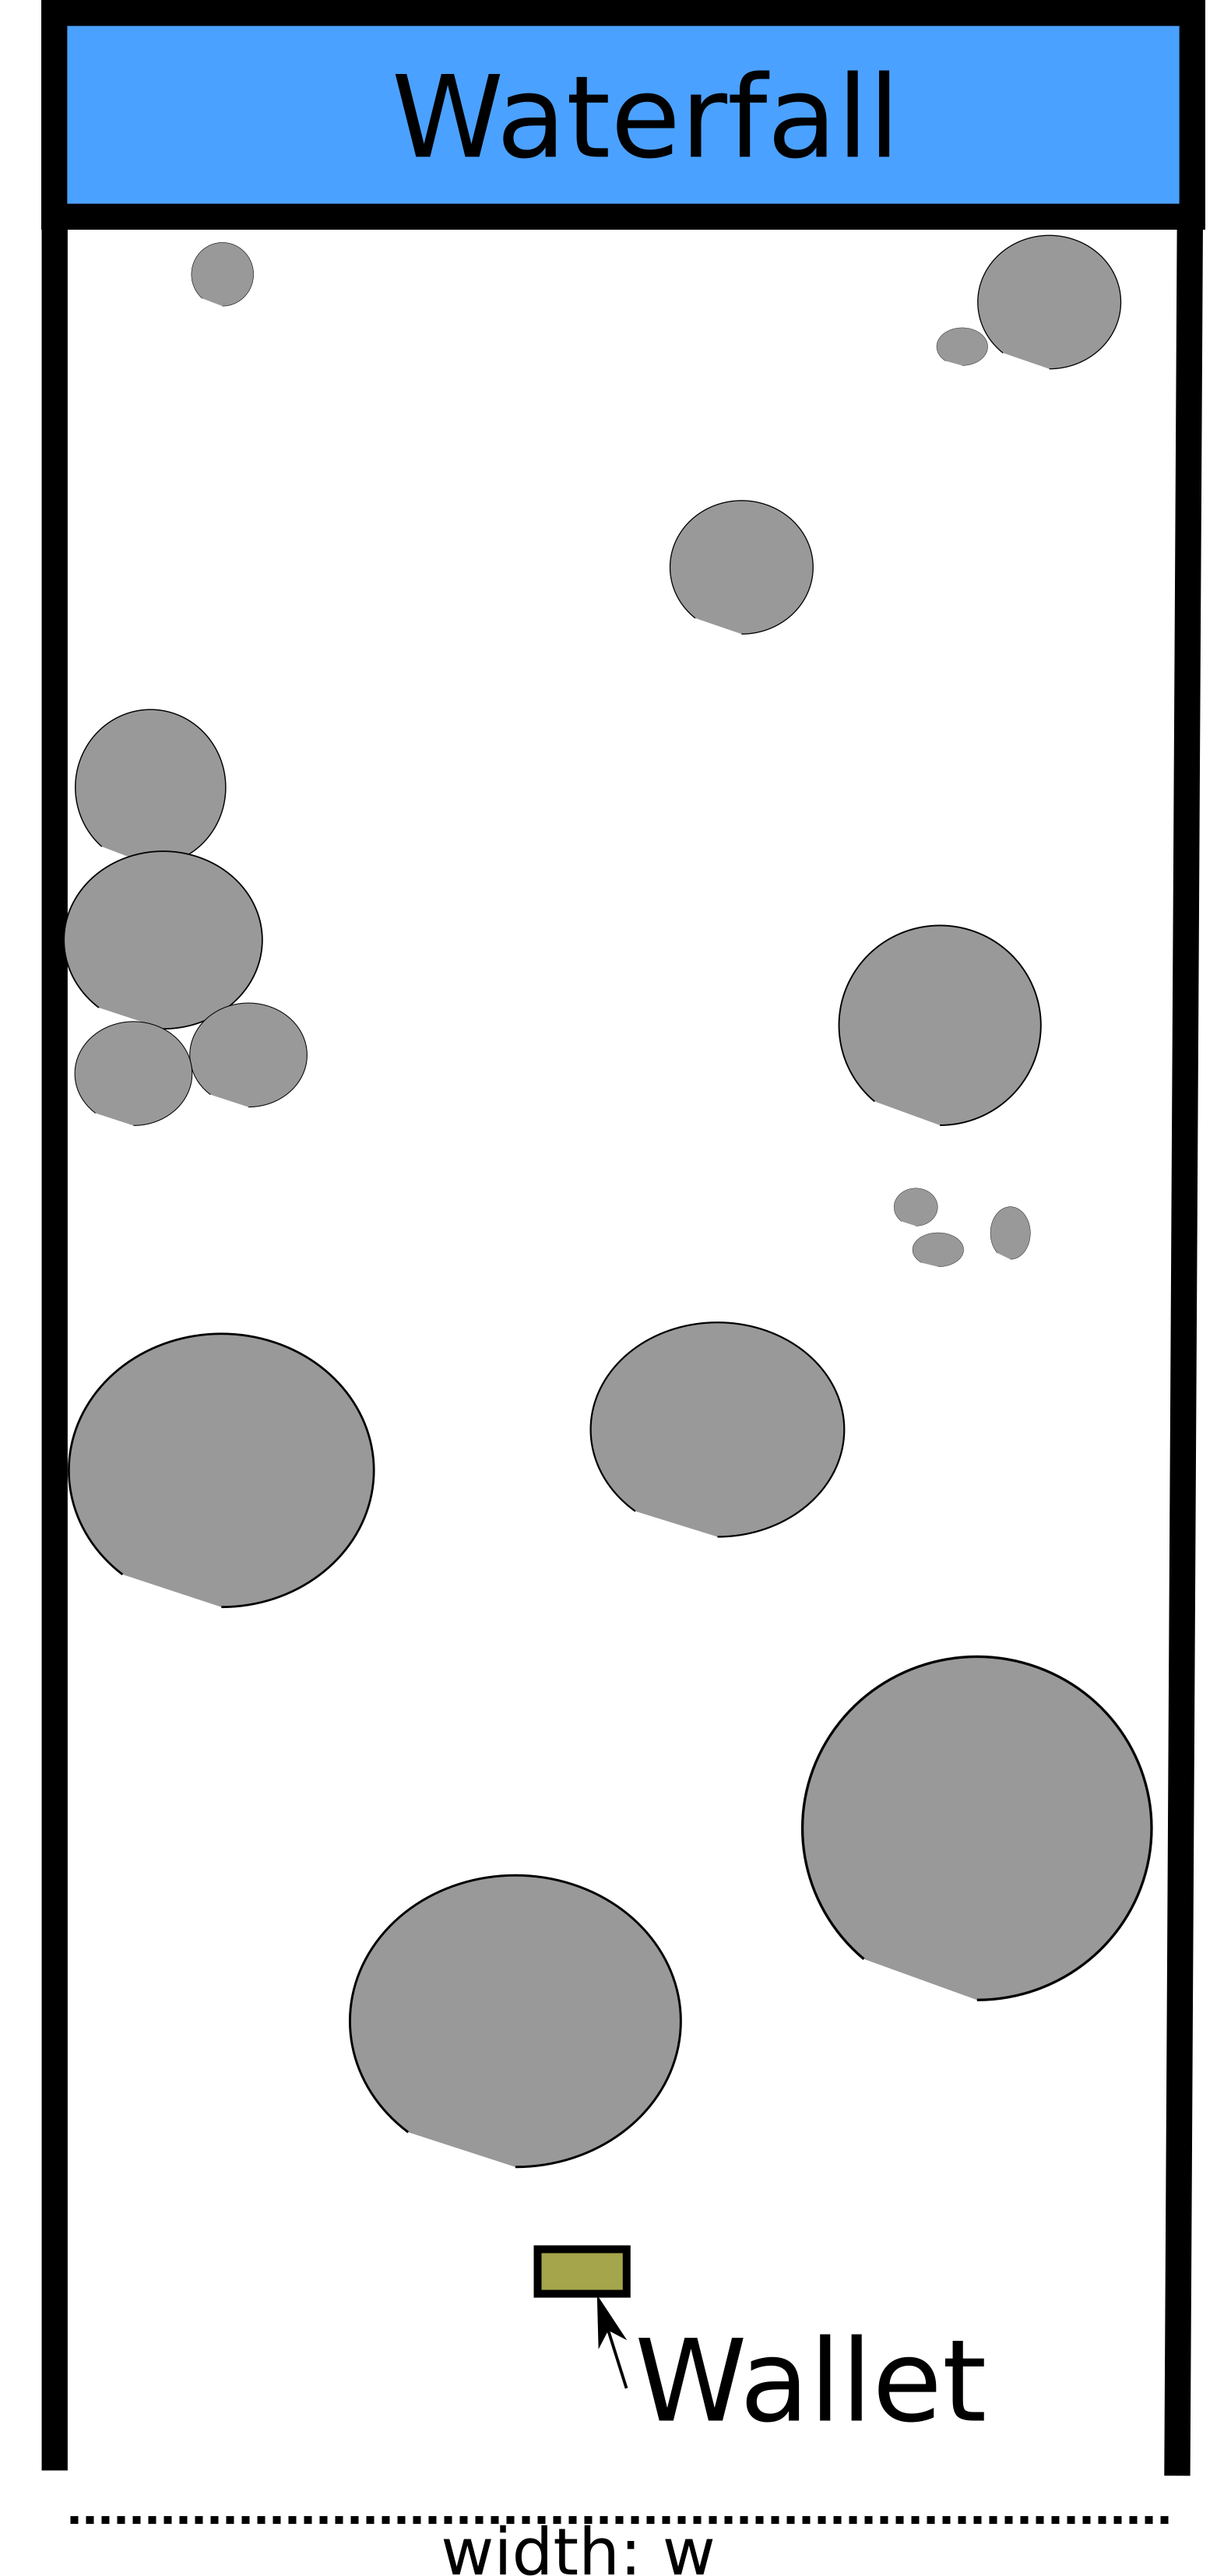
\includegraphics[height=10cm]{images/graphic_river}
\label{fig:sp500_long_results_zoomed}
\end{center}

Note:
\\
Assume that your wallet is capable of manoeuvring between any arbitrarily small gap formed between any two rocks and that rocks may overlap.
\\
Assume that you wallet is capable of temporarily flowing upstream around rocks. 
\\
Assume that the rocks are tall enough that they go from the bottom of the river to above the water... IE you can't possibly go over the rocks. 
\end{problemDescription}

\needspace{5em}
% Specific input definition
% Includes what is being taken as input, and in what format
\begin{inputDescription}
Each case will begin with an input containing an integer, $W$ representing the river width and $N$ being the number of rocks in the river. $0 \leq W \leq 100, 0 \leq N \leq 100$
The following N lines each contain 3 space separated doubles $x_i y_i r_i$, where $x_i$ and $y_i$ represent the x and y coordinates of the ith rock and $r_i$ is the radius of the ith rock. Note that $0 \leq x_i \leq W$, $ 0 \leq y_i \leq 100$, $ 0 < r_i \leq \frac{W}{2}$
Input is finished once the width and number of rocks are both 0. i.e, you read a line: 0 0.
\end{inputDescription}

\needspace{5em}

% Specific output definition
% Includes what should be printed, and in what format
\begin{outputDescription}
Output TRUE if your wallet will go off the waterfall (in any possible way)
Output: FALSE if your wallet is completely safe, that is there is no possible way for it to reach the waterfall.
\end{outputDescription}

\begin{sampleInput}
10 5
1 3 1
8 2 1
5 5 2
2 8 2
9 8 1.5
10 3
0 5 2
4 5 2
8 5 2
0 0
\end{sampleInput}
\begin{sampleOutput}
TRUE
FALSE
\end{sampleOutput}

\end{document}
